\chapter{Datos y balance}

\noindent Para que el análisis del impacto del programa de fotocívicas en la seguridad vial de la Ciudad de México sea factible y estadísticamente robusto, es necesario integrar diversos conjuntos de datos abiertos, organizados en tres categorías fundamentales para la inferencia causal: \textit{treatment}, \textit{outcomes} y \textit{covariates}. El tratamiento se define a partir de la ubicación geográfica de los 113 radares de velocidad registrados por la Secretaría de Seguridad Ciudadana (SSC), lo que permite identificar de manera explícita las unidades espaciales intervenidas por la política. En cuanto a los resultados (\textit{outcomes}), estos corresponden a los incidentes viales confirmados en los registros del C5, analizados tanto en números absolutos como en tasas por cada 1{,}000 vehículos. Esta construcción posibilita una desagregación por nivel de severidad, distinguiendo entre incidentes menores (MIN), con lesiones personales (PIC) y aquellos con víctimas fatales (FCS).\\

Las covariables (\textit{covariates}) cumplen un papel central en el control de los factores que influyen en la asignación de las cámaras y en la garantía de comparabilidad entre unidades mediante el cálculo del \textit{propensity score}. Para ello, se consideran atributos estáticos, que describen la configuración física e invariable de la red vial (jerarquía, número de carriles, sentido y nivel de la traza), así como variables que cambian en el tiempo, empleadas como \textit{proxies} de movilidad para capturar las variaciones en la exposición vehicular asociadas a la pandemia de COVID-19. En particular, la integración de la afluencia diaria del Metro y los volúmenes de tránsito mensual reportados por la SICT contribuye a mitigar sesgos derivados de choques exógenos, y sienta las bases para la implementación de un diseño de diferencias en diferencias aplicado sobre una muestra emparejada con soporte común.

\section{Tratamiento: Programa de Fotocívicas}
El objetivo central de este análisis es identificar el efecto causal de las cámaras de velocidad sobre el número de incidentes viales en la Ciudad de México. Para ello, resulta indispensable contar con la ubicación geográfica precisa de los radares, ya que estos puntos determinan la delimitación de las áreas consideradas como unidades tratadas y sirven como base para la construcción de las unidades de control en el modelo de emparejamiento. A diferencia del esquema previo de fotomultas, la ubicación de estos dispositivos es de acceso público, decisión que se alinea con la naturaleza preventiva del programa de fotocívicas, vigente desde el 22 de abril de 2019. Esta transparencia busca propiciar un cambio genuino en las conductas de los conductores al incentivar el respeto a los límites de velocidad mediante la localización explícita de los equipos, privilegiando la educación vial por encima de la recaudación económica.\\

De acuerdo con los registros de la Secretaría de Seguridad Ciudadana (SSC), el tratamiento se define a partir de un total de 113 radares de velocidad distribuidos en las principales vialidades de la ciudad. La información se obtiene del conjunto de datos \textit{``Fotocívicas (Ubicación)''}, publicado en la Plataforma de Datos Abiertos de la Ciudad de México y actualizado por última vez el 6 de julio de 2023. Este conjunto proporciona variables clave para el análisis geoespacial, entre ellas el nombre de la vialidad, el sentido de circulación sobre el cual opera la cámara y sus coordenadas exactas (latitud y longitud). A partir de estos insumos se define operativamente la variable binaria \texttt{has\_camera} a nivel de celda o área circular, lo que permite identificar la exposición espacial al tratamiento y sienta las bases para la posterior implementación del diseño de diferencia en diferencias.

% aquí está pendiente además mostrar cómo se ve un ejemplo concreto de una unidad tratada y la construcción de sus controles aledaños para que la gente pueda entender a qué es a lo que me estoy refiriendo. También falta detallar que has camera es una variable binaria con valores 0 y 1, para cuando no tienen cámara de velocidad y cuando sí la tienen respectivamete. 

\section{Covariables Geográficas, Estructurales y de Movilidad}
Para mitigar el sesgo de selección inherente al programa de Fotocívicas -- donde los radares se ubican estratégicamente en tramos con mayor siniestralidad, altos volúmenes de traslado y recurrente incumplimiento de límites de velocidad -- es necesario controlar por las características estructurales de la vía. A continuación se describen las covariables de los atributos físicos de la red vial, construidas a partir del conjunto de datos \textit{Vialidades primarias de la Ciudad de México} proporcionado por la Secretaría de Movilidad (SEMOVI). 

\subsubsection{Atributos físicos de la red vial}

\begin{itemize}
    \item \textbf{Número de vialidades (\textit{n\_vialidades}):} 
    Esta variable contabiliza el número de ejes viales únicos que intersectan cada unidad de análisis. Permite controlar por la densidad de la red y la complejidad de la conectividad local, factores que elevan la probabilidad de conflictos vehiculares y, por ende, la probabilidad de que la autoridad asigne una cámara en dicho punto.

    \item \textbf{Capacidad de la vía (\textit{max\_carriles}):} 
    Corresponde al número máximo de carriles observado entre las vialidades de la celda. Se utiliza como un proxy de la capacidad vial y del volumen potencial de tránsito. Las vías con mayor número de carriles suelen permitir velocidades más altas y concentrar flujos masivos, lo que las hace candidatas prioritarias para el tratamiento.

    \item \textbf{Sentido de circulación (\textit{both\_directions}):} 
    Indicador binario que señala la presencia de al menos una vialidad de doble sentido en el área. La direccionalidad influye en la siniestralidad al introducir maniobras de giro y potenciales conflictos frontales o laterales que no existen en vías de un solo sentido.

    \item \textbf{Jerarquía vial (\textit{via\_primaria}):} 
    Variable dicotómica que indica si la unidad contiene vías clasificadas como primarias. Según el Reglamento de Tránsito, estas vías tienen funciones de flujo continuo o controlado por semáforos y límites de velocidad específicos (50 km/h), lo que las define como el objetivo central del programa sancionatorio.

    \item \textbf{Vías de acceso controlado (\textit{via\_acc\_cont}):} 
    Identifica la presencia de corredores con regulación y geometría específica, como entradas y salidas mediante carriles de aceleración y desincorporación. Estas vías (con límites de hasta 80 km/h) presentan niveles de riesgo y exposición distintos a las arterias convencionales, influyendo directamente en la decisión gubernamental de monitoreo.

    \item \textbf{Complejidad vertical (\textit{max\_nivel}):} 
    Representa el nivel máximo sobre el suelo (\textit{z-order}) de las vialidades presentes. Esta covariable es crítica en la Ciudad de México para encapsular la dinámica de vías de múltiples niveles, como el segundo piso del Periférico, donde los riesgos de siniestralidad y la visibilidad de los radares difieren del nivel de calle.

    \item \textbf{Longitud vial acumulada (\textit{road\_length\_m}):} 
    Mide la cantidad total de metros de red vial contenidos dentro del área de estudio. El control por longitud permite realizar un emparejamiento basado en la exposición física: una alta concentración de metros de vía suele corresponder a cruces de grandes avenidas o nudos viales complejos, los cuales implican un mayor flujo vehicular y una probabilidad intrínsecamente más alta de colisiones.
\end{itemize}

Estas variables operan como controles fijos en el cálculo del \textit{propensity score}, garantizando que la comparación se realice entre tramos viales con estructuras físicas, capacidades y jerarquías comparables, aislando así el efecto del radar de la peligrosidad natural del diseño vial.

\subsubsection{Proxies de movilidad y exposición}

Para capturar la dinámica de movilidad urbana y mitigar las distorsiones causadas por cambios en el flujo de personas, especialmente ante choques exógenos, se incorporaron \textit{proxies de movilidad} basados en el sistema de transporte masivo de la ciudad. El uso de estos indicadores es fundamental para controlar el choque exógeno de la pandemia de COVID-19, la cual provocó una reducción en la movilidad de entre el 40\% y el 60\%, permitiendo velocidades de circulación más altas y una recomposición en la severidad de los incidentes viales. A continuación se detalla la construcción y el procesamiento de estas fuentes.

\paragraph{Fuentes de datos}

\begin{itemize}
    \item \textbf{Coordenadas de estaciones de metro (\textit{metro coordinates}):} 
    Ante la ausencia de un registro unificado con precisión geográfica para todas las estaciones, se generó un conjunto de datos de creación propia mediante la extracción automática de información de Google Maps. Este proceso consistió en la búsqueda sistemática de cada una de las 167 estaciones del sistema para registrar sus coordenadas geográficas exactas (latitud y longitud), permitiendo así la georreferenciación precisa de la infraestructura de transporte dentro de la cuadrícula de análisis.

    \item \textbf{Afluencia del metro:} 
    Se utilizó el conjunto de datos \textit{``Afluencia diaria del metro CDMX''}, proporcionado por la Secretaría de Movilidad (SEMOVI), el cual registra el volumen diario de usuarios por línea y estación. Estos datos, con cobertura desde enero de 2010 hasta abril de 2025, se unieron (\textit{join}) con las coordenadas geográficas previamente obtenidas para localizar los flujos de personas en el espacio urbano.
\end{itemize}

\subsubsection{Construcción de variables para el emparejamiento (\textit{matching})}

Para que estos datos temporales pudieran integrarse en el cálculo del \textit{propensity score} y asegurar que las unidades tratadas y de control fueran comparables en su dinámica de flujo previa a la intervención, se aplicó un proceso de agregación y ``compresión'' de las series históricas. A cada unidad de análisis (celda) se le asignó la información de la estación de metro más cercana, asumiendo que esta es la representación más fiel del flujo humano y la actividad comercial en esa zona específica.

Las variables resultantes para el \textit{matching}, calculadas exclusivamente con datos previos al inicio del programa (22 de abril de 2019), son las siguientes:

\begin{itemize}
    \item \textbf{Distancia a la estación (\textit{distance\_to\_station}):} 
    Mide la distancia en metros desde el centroide de cada celda a la estación de metro más cercana, sirviendo como un control de proximidad a nodos de alta actividad.

    \item \textbf{Media de afluencia mensual (\textit{mean\_afluencia\_mensual}):} 
    Representa el nivel promedio de demanda y exposición peatonal/vehicular de la zona durante el periodo preintervención.

    \item \textbf{Desviación estándar de la afluencia (\textit{std\_afluencia\_mensual}):} 
    Captura la volatilidad o variabilidad de los flujos en la zona, permitiendo emparejar celdas que no solo comparten niveles de tráfico similares, sino también patrones de estabilidad o fluctuación parecidos.
\end{itemize}

Este tratamiento de los datos permite que el modelo de evaluación asuma que, tras el emparejamiento, las diferencias en la siniestralidad no son producto de variaciones locales en la movilidad o del impacto diferenciado de la pandemia, sino del efecto causal de los radares de velocidad.

\subsubsection{Estaciones de conteo permanente de tránsito}

Para captar la exposición vehicular y el volumen de tráfico —factores que con frecuencia se omiten en evaluaciones locales de seguridad vial— incorporo datos de las \textit{estaciones de conteo permanente} mantenidas por la Secretaría de Infraestructura, Comunicaciones y Transportes (SICT).

\paragraph{Obtención y procesamiento de los datos}

La información se extrajo de los informes anuales de \textit{Datos Viales} (con cobertura de 2015 a 2024), los cuales reportan el volumen total anual y la distribución porcentual mensual para distintos puntos de la red carretera. Dado que estos datos se publican en archivos PDF no estructurados y con identificadores inconsistentes, fue necesario desarrollar una metodología de procesamiento que garantizara la integridad de la información. 

Este proceso incluyó la localización de las tablas relevantes a partir de coordenadas geográficas y tramos carreteros, el uso de un \textit{large language model} (LLM) para extraer las cifras a un formato estructurado y la validación manual para seleccionar las 20 estaciones que permanecieron operando de manera continua durante todo el periodo de análisis.

\paragraph{Contribución a la literatura}

El uso de estas series representa una contribución importante a la literatura de seguridad vial en la Ciudad de México. Estudios previos —como Quintero et al.\ (2022) o Madrigal y Rodríguez (2021)— no utilizaron estos conjuntos de datos específicos de la SICT para controlar el choque exógeno de la pandemia de COVID-19 ni las variaciones generales en la exposición. Al integrar estas cifras, el presente estudio incorpora un control más robusto para las caídas abruptas en el tráfico (estimadas entre 40\% y 60\% durante 2020) que, de otra forma, sesgarían la estimación del impacto de los radares de velocidad.

\paragraph{Resolución espacial y estandarización}

Una limitación importante de la fuente es que las estaciones de conteo disponibles se ubican principalmente en las periferias de la ciudad, como plazas de cobro y accesos carreteros, y no en el tejido urbano central. Idealmente, el análisis utilizaría datos de flujo capturados directamente en cada una de las celdas de la cuadrícula de estudio; sin embargo, la ausencia de sensores urbanos de acceso público impide esta aproximación.

En consecuencia, este trabajo aplica una \textit{``estandarización a nivel ciudad''} en lugar de un control de flujo específico por unidad. Esto implica asumir que las fluctuaciones de movilidad observadas en las entradas a la ciudad son un proxy razonable de la dinámica interna del área urbana. Para mitigar el posible error de medición derivado de este enfoque agregado, estas series se complementan con \textit{proxies} de tránsito de mayor resolución, como la afluencia del metro.

\section{Siniestralidad y resultados}

En esta sección se describe la construcción de la variable de siniestralidad y la forma en que se utiliza tanto como resultado principal (\textit{outcome}) como covariable en la fase de emparejamiento (\textit{matching}). Se parte de los registros de incidentes viales del Centro de Comando, Control, Cómputo, Comunicaciones y Contacto Ciudadano de la Ciudad de México (C5), y se detalla el proceso de depuración, clasificación y agregación de la información.

\subsection{Fuente de datos y justificación}

\noindent Los registros de incidentes viales cumplen un doble papel en el análisis. Por un lado, constituyen la variable dependiente principal para estimar el impacto del programa de fotocívicas. Por otro, se utilizan como covariable en el emparejamiento, con el fin de capturar el riesgo base de cada zona antes de la intervención. El Gobierno de la Ciudad de México señaló que la ubicación de las cámaras se definió con base en la incidencia histórica de hechos de tránsito, en particular en tramos con mayor número de muertos y lesionados. En este contexto, resulta indispensable controlar por el historial de siniestralidad para mitigar el sesgo de selección y evitar atribuir a las cámaras diferencias que se explican por condiciones de riesgo preexistentes.\\

La información proviene del conjunto de datos \textit{``Incidentes viales reportados por C5''}. Esta fuente se prefiere frente a los registros de la Secretaría de Seguridad Ciudadana (SSC) por dos razones metodológicas:

\begin{enumerate}
    \item \textbf{Cobertura temporal:} los datos de la SSC solo cuentan con georreferenciación precisa a partir de junio de 2018, lo que impide construir una ventana simétrica de tres años previos y tres posteriores a la implementación de la política. En contraste, el C5 ofrece registros desde diciembre de 2013, lo que permite definir una ventana de análisis más amplia y balanceada.
    \item \textbf{Representatividad:} la base de la SSC se restringe a incidentes con lesionados o fallecidos, mientras que el C5 integra llamadas al 911, activaciones de botones de auxilio y videovigilancia, incluyendo incidentes menores. Excluir estos eventos leves podría sesgar los resultados si la política incide sobre la frecuencia total de percances y no únicamente sobre su gravedad.
\end{enumerate}

\subsection{Depuración y clasificación de incidentes}

El universo inicial de análisis está conformado por 2\,115\,080 registros. A partir de esta base se aplicaron varios filtros para obtener una muestra consistente con los objetivos del estudio. En primer lugar, se conservaron únicamente los folios con código de cierre A (Afirmativo), que identifica incidentes verificados por las autoridades en el lugar de los hechos. Este paso permite eliminar duplicados, falsas alarmas e incidentes externos. En segundo lugar, se restringió la muestra a eventos tipificados como \textit{Accidente}, \textit{Cadáver} o \textit{Lesionado}, descartando otros tipos de llamadas al C5 que no están directamente relacionados con hechos de tránsito. En tercer lugar, se delimitó la ventana temporal para cubrir exclusivamente tres años antes y tres años después de la intervención, es decir, del 22 de abril de 2016 al 21 de abril de 2022.\\

Tras este proceso de depuración, la base analítica final quedó conformada por 432\,707 incidentes. Estos se agrupan en tres categorías mutuamente excluyentes, en línea con los estándares de la literatura internacional orientada a capturar tanto el volumen de choques como su impacto en salud pública:

\begin{itemize}
    \item \textbf{FCS (fatalidad):} incluye 1\,957 incidentes en los que se registró un cadáver en el lugar de los hechos.
    \item \textbf{PIC (lesión personal):} agrupa 191\,681 incidentes en los que la clasificación de alarma fue \textit{Urgencias Médicas}.
    \item \textbf{MIN (menor):} considera 239\,069 incidentes sin lesionados ni fallecidos, usualmente asociados con daños materiales o alcances leves.
\end{itemize}

\subsection{Uso de la siniestralidad en el análisis causal}

Operativamente, la información de siniestralidad se utiliza con dos fines complementarios.

\paragraph{Emparejamiento de unidades}

En la etapa de emparejamiento, se calculan medias y desviaciones estándar mensuales de accidentes por celda durante el periodo pretratamiento (2016--2019). Estas estadísticas permiten que el \textit{propensity score} agrupe celdas con perfiles de riesgo y volatilidad similares antes de la instalación de las cámaras. De esta forma, se reduce la probabilidad de comparar zonas estructuralmente muy distintas en su historial de siniestros.

\paragraph{Estimación de efectos (diferencias en diferencias)}

En la etapa de estimación, se emplea un diseño de diferencia en diferencias. Para ello, los datos se agregan a nivel mensual y por celda, y se construyen dos tipos de indicadores:

\begin{itemize}
    \item conteos absolutos de incidentes en cada categoría (FCS, PIC y MIN);
    \item tasas por cada 1\,000 vehículos, utilizando información independiente de exposición vehicular.
\end{itemize}

Esta estrategia permite evaluar el comportamiento de la siniestralidad tanto en términos de frecuencia como de gravedad relativa, y determinar si las cámaras de velocidad lograron reducir los incidentes viales de manera localizada, una vez controlado el riesgo base y la exposición al tráfico.

\section{Pruebas de balance}
Para garantizar la validez interna de las estimaciones y asegurar que las diferencias observadas en la siniestralidad puedan interpretarse de manera causal, es fundamental verificar la calidad del procedimiento de emparejamiento. Un proceso de matching exitoso es aquel que logra mitigar el sesgo de selección, construyendo un contrafactual donde las unidades de control y tratamiento sean estadísticamente comparables en función de sus covariables observables.

\subsection{Supuesto de soporte común y recorte de la muestra}
Un requisito central de la estrategia de identificación es la satisfacción del supuesto de \textbf{soporte común} (\textit{common support}). Este supuesto existe que, para cada valor del \textit{propensity score} observado en el grupo tratado, exista un conjunto suficiente de unidades de control con probabilidades de tratamiento similares. La ausencia de solapamiento en las distribuciones de los puntajes de propensión invalidaría la comparación, al intentar emparejar unidades estructuralmente distintas. 

El cálculo del \textit{propensity score} se realizó integrando aquellas dimensiones críticas que, de acuerdo con la lógica oficial, determinan la asignación de los radares de velocidad: atributos físicos de la red vial, proxies de movilidad y exposición vehicular, así como el historial de siniestralidad previo al tratamiento.  
\begin{figure}[htbp]
    \centering
    \caption{Soporte del Propensity Score por Distancias}
    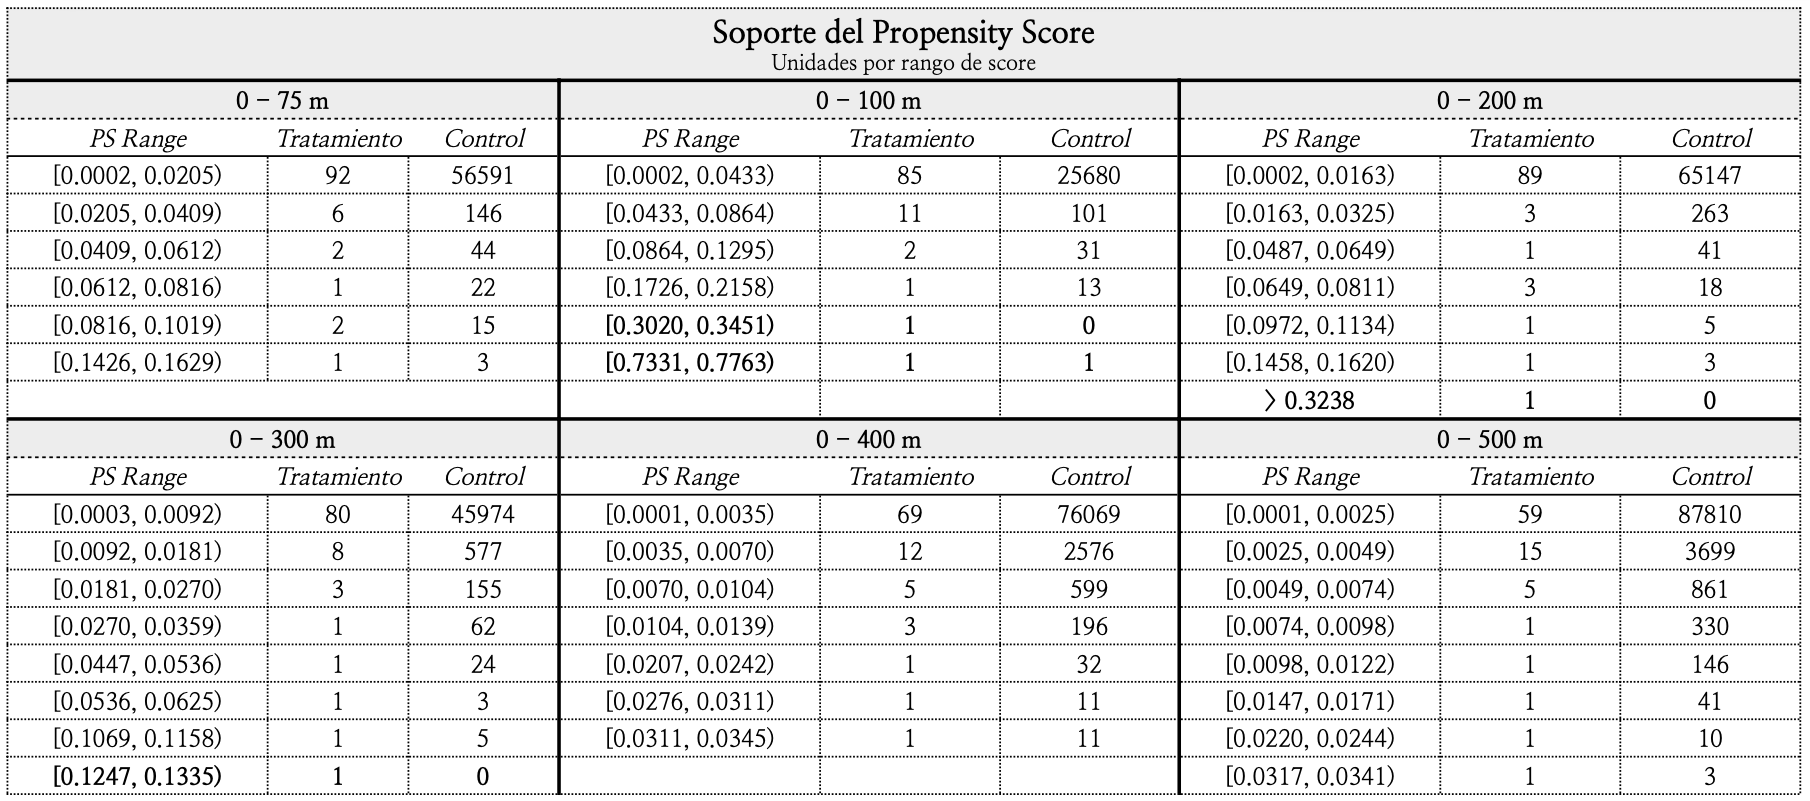
\includegraphics[width=\textwidth]{Imagenes/soporte-propensity-score.png}
\end{figure}

Con el objetivo de robustecer el emparejamiento, se evaluó la densidad de controles disponibles para cada rango del propensity score. \footnote{Para el cálculo de los rangos evaluados se consideró el rango de valores de los propensity scores de las unidades de control, partiendo dicho rango en 20 bins del mismo tamaño, y contando cuántas unidades tenían un propensity score en dicho rango} Se estableció un umbral mínimo de tres unidades de control por cada unidad tratada dentro de un mismo rango para poder proceder con el emparejamiento; en caso contrario, la unidad tratada se excluye del análisis. Tras aplicar este procedimiento de \textit{trimming}, se identificaron cuatro casos específicos donde fue necesario restringir la muestra: 
 
\begin{itemize}
    \item \textbf{Distancia de 50 metros}: Se excluyeron las unidades tratadas con un \textit{propensity score} mayor o igual a \textbf{0.3020}
    \item \textbf{Distancia de 200 metros}: Se excluyeron las unidades tratadas con un \textit{propensity score} mayor o igual a \textbf{0.3238}
    \item \textbf{Distancia de 300 metros}: Se excluyeron las unidades tratadas con un \textit{propensity score} mayor o igual a \textbf{0.1247}
\end{itemize}

Para el resto de las distancias y rangos analizados, las distribuciones muestran un solapamiento adecuado, lo que permite construir un universo de controles representativo y similar a las unidades tratadas sin necesidad de exclusiones adicionales

\subsection{Evaluación del balance mediante SMD}

Una vez definida la muestra con soporte común, se procedió a verificar la calidad del balance entre las unidades tratadas y sus respectivos contrafactuales. Para este propósito, se utilizó la \textit{Diferencia de Medias Estandarizada} (\textit{Standardized Mean Difference}, SMD), un indicador robusto que permite cuantificar el desequilibrio de las covariables sin depender del tamaño de la muestra. De acuerdo con el consenso en la literatura de inferencia causal, se considera que un proceso de emparejamiento es exitoso cuando los valores absolutos de SMD se sitúan por debajo del umbral de $0.1$, lo que garantiza que las unidades son estadísticamente comparables y que el sesgo de selección ha sido mitigado.

La Figura~[3.2] resume este diagnóstico para los distintos radios analizados (desde $37.5$ hasta $250$ metros), comparando la SMD antes (\textit{unadjusted}) y después (\textit{matched}) del procedimiento de emparejamiento.

\begin{figure}[htbp]
    \centering
    \caption{Comparación de SMD para radios evaluados}
    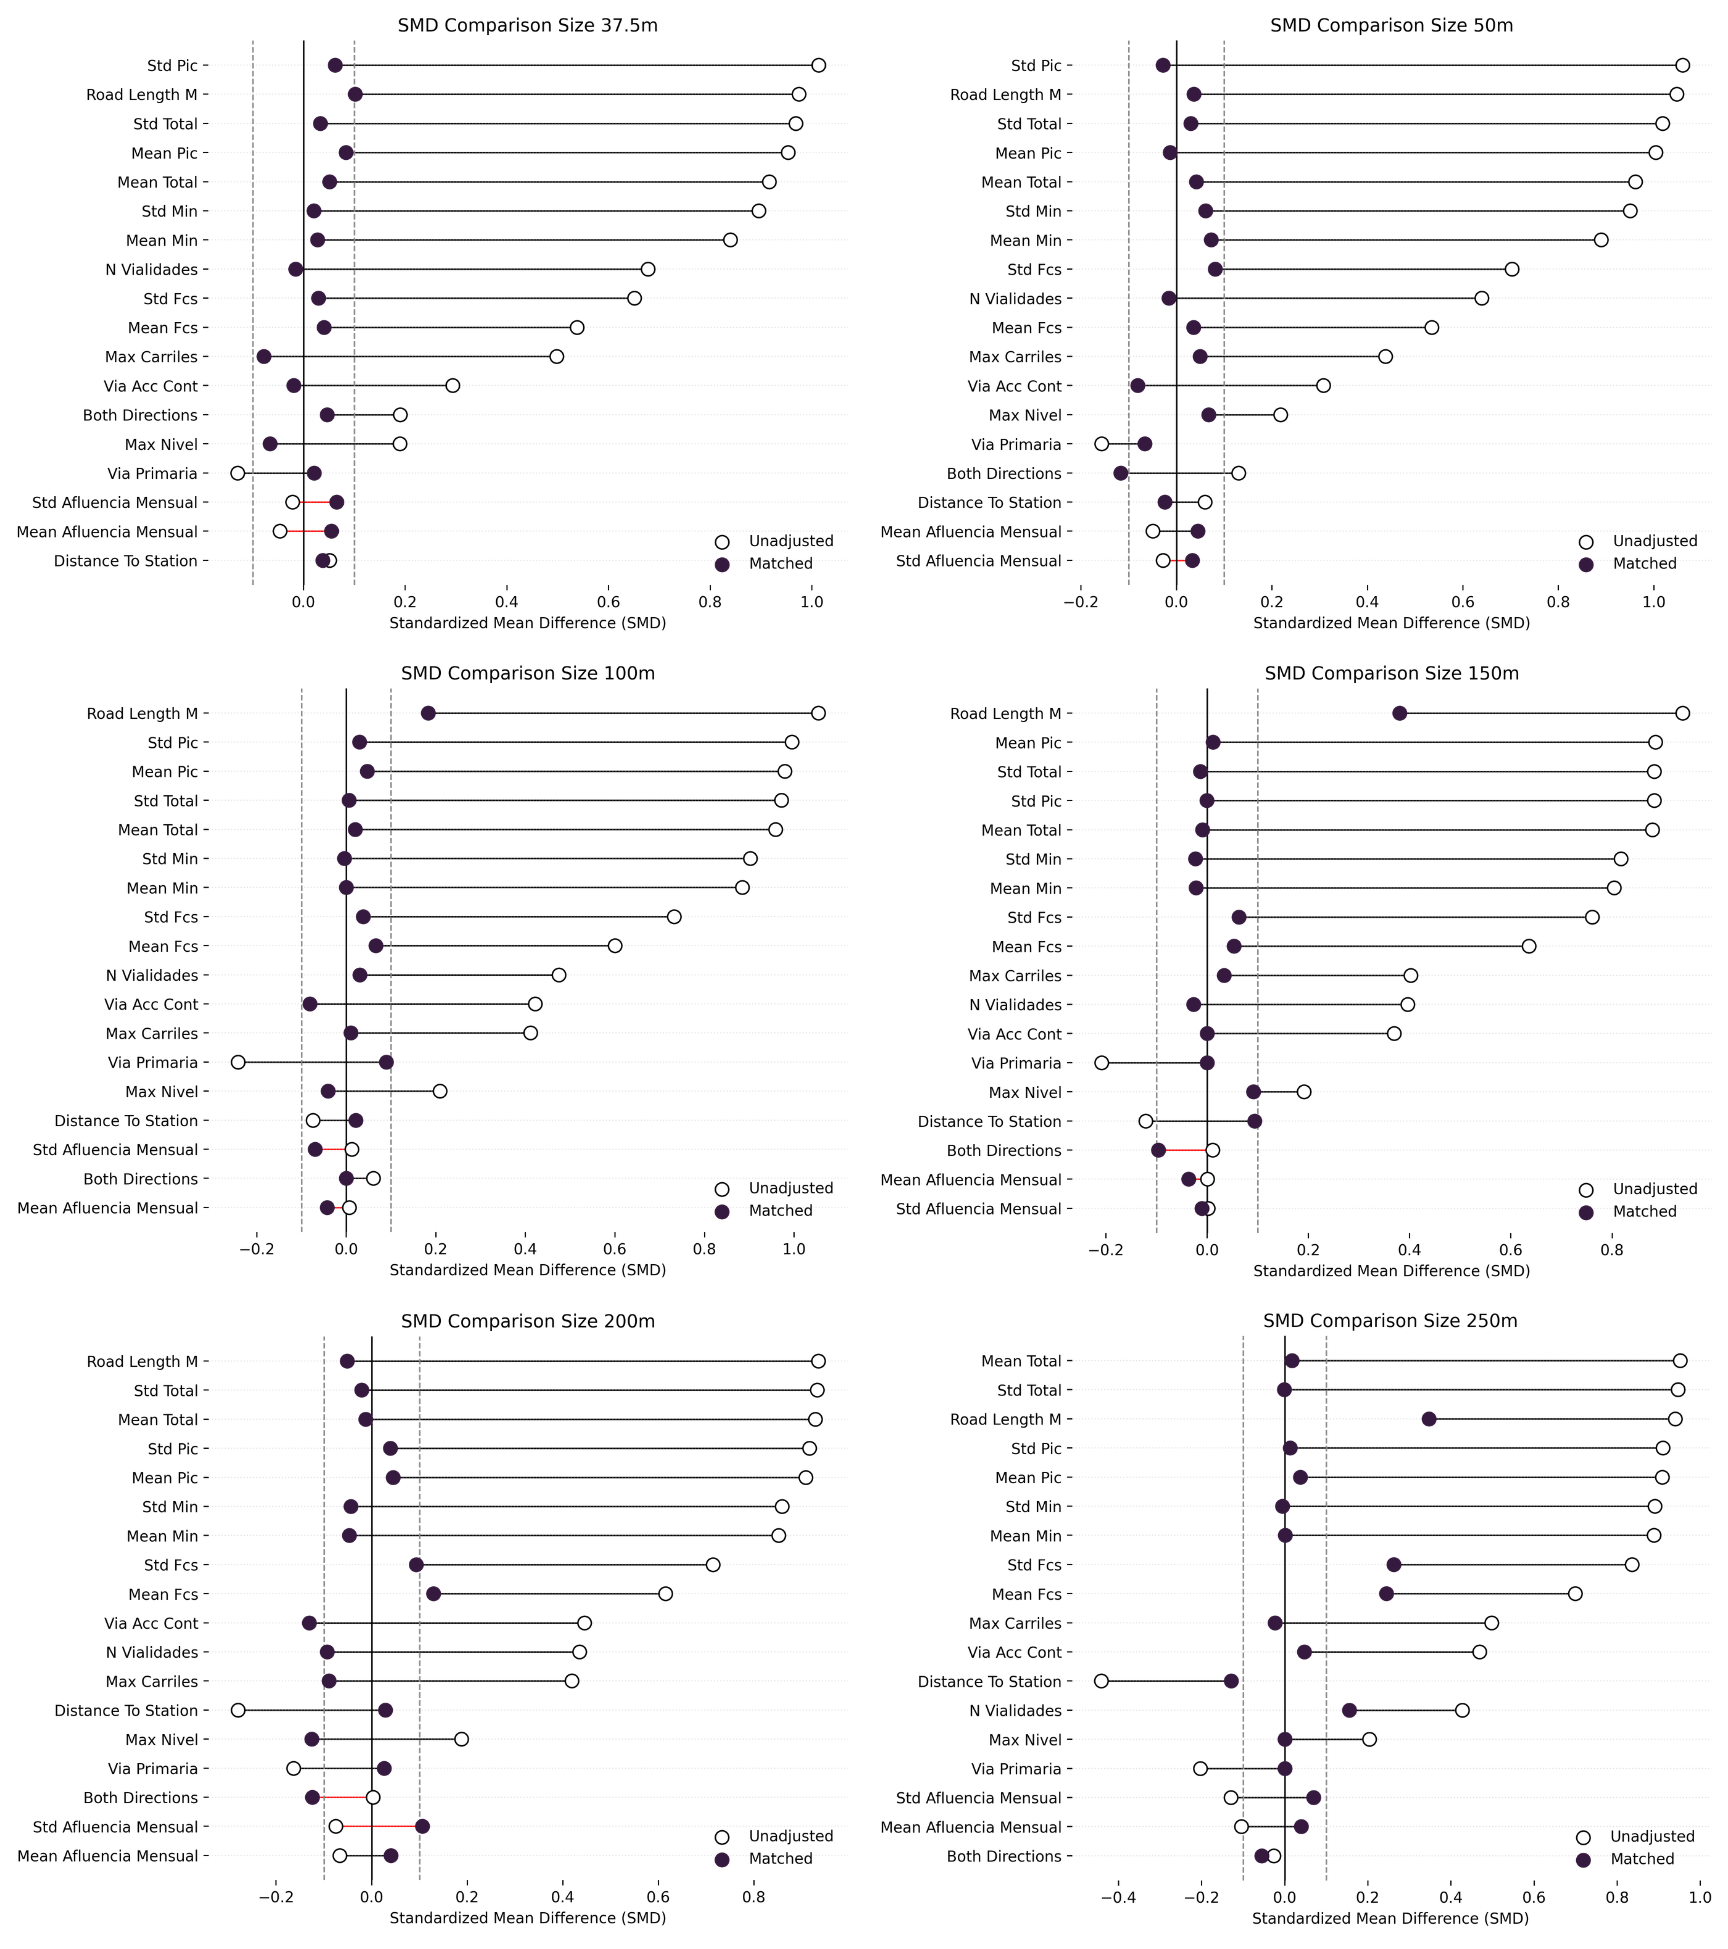
\includegraphics[width=\textwidth]{Imagenes/smd-comparisons.png}
\end{figure}

De manera consistente en todas las especificaciones, se observa una reducción sustancial en los valores de SMD para la mayoría de las covariables, lo que confirma que el algoritmo de \textit{nearest neighbor matching} logró construir grupos de control significativamente más similares a los tratados en comparación con la muestra original.

\begin{itemize}
    \item \textbf{Radios de alta precisión (37.5 m, 50 m y 100 m):} En estas escalas, el balance alcanzado es óptimo. En el radio de $50$ metros, prácticamente todas las variables —incluyendo el historial de siniestralidad pretratamiento y los \textit{proxies} de movilidad— se sitúan cerca del valor cero. Para las distancias de $37.5$ y $100$ metros, si bien variables como la distancia a estaciones de metro o la jerarquía vial presentan desbalances residuales mínimos, el SMD medio posterior al emparejamiento se mantiene por debajo del umbral crítico de $0.1$.
    \item \textbf{Radios intermedios (150 m y 200 m):}  A medida que el área de influencia se expande, la complejidad de las unidades espaciales aumenta. No obstante, el emparejamiento logra estabilizar la mayoría de las dimensiones críticas. En el radio de $200$ metros se observa una mayor dispersión en variables estructurales como el sentido de circulación (\textit{Both Directions}) y el nivel de la traza (\textit{Max Nivel}), aunque el balance global sigue permitiendo comparaciones válidas.
    \item \textbf{Radio de 250 m:}  En esta escala se registra la mayor variabilidad residual. Debido a la extensión del área, las unidades tratadas presentan configuraciones viales más heterogéneas, lo que dificulta encontrar controles perfectos en todas las dimensiones simultáneamente. Sin embargo, aun en este caso, el procedimiento de \textit{matching} reduce drásticamente el sesgo observado en la muestra original, mejorando la comparabilidad de las distribuciones respecto al escenario sin ajuste.
\end{itemize}

En conclusión, los diagnósticos de balance confirman que la estrategia de identificación es robusta. Aunque en los radios de mayor tamaño existen variables que superan levemente la cota de $0.1$, la mejora generalizada en la similitud de las covariables permite proceder con la estimación de los efectos mediante modelos de \textit{diferencia en diferencias}, bajo el supuesto de que las diferencias observadas en la siniestralidad no son producto de disparidades estructurales preexistentes entre los grupos, sino del efecto causal de los radares de velocidad.